\documentclass[12pt]{article}
\usepackage[paperheight=210mm,paperwidth=148mm,top=2cm,bottom=2cm,left=1cm,right=1cm]{geometry}  % A5 paper
\usepackage{background}
\backgroundsetup{
scale=1,
opacity=0.1,
angle=0,
color=black,
contents={%

\includegraphics[width=\paperwidth]{background}
}
}
%%%%%%%%%%%%%%%%%%%%%%%%%%%%%%%%%%%%%%%%
\usepackage[utf8]{inputenc}
\usepackage{titlesec}
%\usepackage[all]{hypcap}
\usepackage{multirow}
%\usepackage{tikz}
\usepackage{ctable}
%%%%%%%%%%%%%%%%%%%%%%%%%%%%%%%%%%%%%%%%
\renewcommand{\familydefault}{\sfdefault}
% \titleformat{\chapter}[display]
% {\bfseries\LARGE\sffamily}{\chaptertitlename}{10pt}{\LARGE}
% \titlespacing*{\chapter}{0pt}{10pt}{10pt}
% \numberwithin{table}{chapter}


\begin{document}
% Cover
\newgeometry{left=0cm, bottom=0cm, top=0cm, right=0cm}
\thispagestyle{empty}
\noindent  % To remove the unwanted white space.

\includegraphics{capa}
\NoBgThispage

\clearpage

\restoregeometry

\newpage

% TODO Adicionar carta do organizador.
% A carta deve conter uma visão geral do event.

Att,
Organizador.

\newpage

\section*{Programa}

O programa divulgado para os participantes foi

% TODO Adicionar link para slides ou apresentação.
\begin{tabular}{cll}
  Horário & Título & Instrutor \\
  9h-10h & SciTools Install Fest: Python - Anaconda, LaTeX, Git & \\
  10h10-12h10 & Introdução ao Python & Mário Sergio \\
  12h10-13h40 & Almoço \\
  13h40-14h40 & LaTeX - Automatizando a criação de PDFs com LaTeX+Python & Melissa Mendonça \\
  14h50-15h50 & Git/GitHub & Matheus Braun \\
  16h00-17h00 & Open Science / Ciência Aberta & Ivan Ogassavara \\
\end{tabular}

% TODO Adicionar atrasos que ocorreram.

\begin{figure}[!htb]
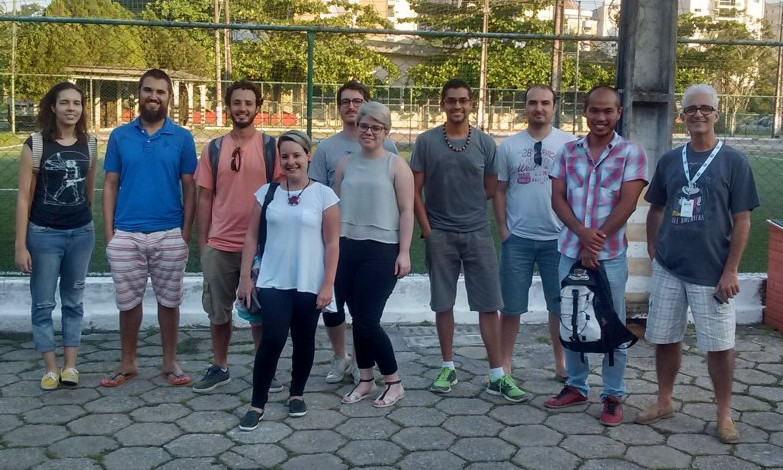
\includegraphics[width=\textwidth]{../../media/photos/pre4-cut}
\caption{Instrutores}
\end{figure}

\newpage

\section*{Público}

Entre os dias 8 de Abril e 16 de Abril (quando o evento foi realizado)
tivemos 29 inscritos (26 homens e 3 mulheres).

\begin{figure}[!htb]
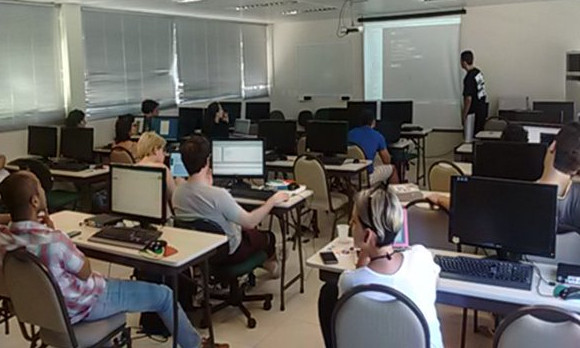
\includegraphics[width=\textwidth]{../../media/photos/pre0-cut}
\caption{Instrutores}
\end{figure}

% TODO Adicionar mais informações sobre os inscritos.

\newpage

\section*{Repercussão}

% TODO Adicionar informações sobre o que aconteceu nas redes sociais
% e do feedback que a organização teve (oral ou escrito).

\newpage

\section*{Finanças}

% TODO Adicionar todos os gastos da organização
% incluindo passagens de ônibus e ou gasolina.

\end{document}
